%!TEX root = paper.tex

\section{Use case}
\label{sec:use_case}

The intention of this paper was to show the advances made regarding web service discovery and consumption through the two artifacts developed as part of our research. While these artifacts may be deployed and used separately by third-party applications, they were originally developed to form the backbone of the FAST platform~\cite{hoyer2009fast}.
FAST constitutes a novel approach to application composition and business process definition from a top-down user-centric perspective. Therefore, it is aimed at allowing users (mainly business users at the management level, without programming experience) to create their own situational applications by visually combining different components, or building blocks, such as graphical forms and back-end services in terms of their inputs and outputs. These two components, as described in Sects. 3 and 4, are fully integrated and present a high cohesion with the rest of the components of the FAST architecture (see Fig.~\ref{fig:fast_architecture}). 

\begin{figure}[ht]
  \begin{center}
    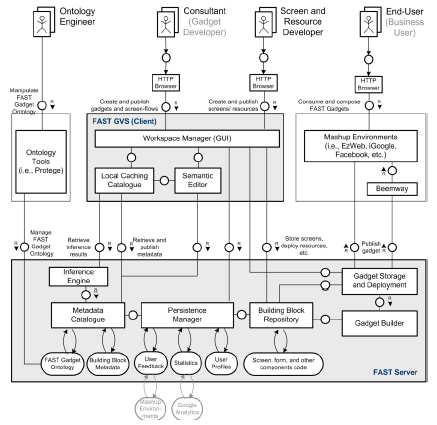
\includegraphics[width=.9\linewidth]{images/fast_architecture.png}
    \caption{Overview of the FAST architecture}
    \label{fig:fast_architecture}
  \end{center}
\end{figure}

In order to facilitate a better understanding of the use case, we will describe a number of concepts related to FAST in this section. A \emph{gadget} is the end product of the platform, aimed to be used in a specific mashup platform. Within FAST, the platform-independent gadget is called \emph{screenflow}, which comprises a set of domain-specific \emph{screens} connected through their \emph{pre-} and \emph{post-conditions}. A screen is the most complex building block fully functional by itself. It is composed by a \emph{form} conveying the graphical interface, and a set of \emph{operators} and \emph{back-end services}, wrapped into so-called \emph{service resources}.

Then, the web service wrapper tool, which is used to create the formal definitions of back-end services, transforming them into building blocks to be stored and reused within the FAST platform. It is integrated into the graphical IDE, and for the storage interacts with the catalogue, where the formal service descriptions and the executable code encapsulating the service behaviour is stored.

The publishing platform presented, called ``Resource Catalogue'' within the FAST platform, covers several important purposes:
\begin{description}
	\item[Publication and search of gadgets] The output of the FAST IDE are gadgets, which are self-contained and ready to use for users. They need to be made available for download, as well as being discover according to their formal description.
	\item[Publication and search of building blocks] Every single component or building block definition is stored in the catalogue and it provides powerful ways of searching, recommendation and planning. 
	\item[Storage and indexing of user profiles and histories] Each user of the FAST platform will have a representation in the catalogue, thus making it possible for the IDE to make informed guesses about what they want in a particular situation, based on their previous behaviour.
	\item[Facilitate ontology mediation] Because FAST allows the integration of third-party external services, it is not always guaranteed that all the data coming from a service is directly compatible with the FAST platform. In such cases, mediation between the different ontologies is necessary. The catalogue provide some grade of mediation functionality.
\end{description}
